\chapter{基于主动学习的选点}

基于机器学习的视频压缩中关键性的一个步骤就是选取最具有代表性的点。在本
节中我们将会介绍一种基于主动学习的选点方法。这种主动学习的方法使用的损
失函数和上一小节中介绍的半监督学习算法的损失函数完全相同。具体地说,我
们希望使用这种方法选出来的点用于训练可以最小化预测误差。

\section{Bias和Variance的分析}

因为$y_i=\textbf{a}^T \mathbf{z}_i+\epsilon$,我们有$\mathbf{y}=Z^T
\mathbf{a}+\pmb{\epsilon}$,其中$\pmb{\epsilon}=(\epsilon, \cdots,
\epsilon)^T$。显然$E(\pmb{\epsilon}) = \mathbf{0}$,其
中$\mathbf{0}=(0,\cdots,0)$。我们定义
\begin{equation}\label{eqn:hessian-LapRLS}
H=ZZ^T + \lambda_1 XMX^T + \lambda_2 I
\end{equation}
\begin{equation}\label{eqn:lambda-LapRLS}
\Lambda=\lambda_1 XMX^T + \lambda_2 I.
\end{equation}
其中$H$是损失函数的黑塞矩阵。系数向量$\mathbf{a}$的估计值的bias可
以由以下的式子计算出来:
\begin{eqnarray}
% \nonumber to remove numbering (before each equation)
&& E(\widehat{\textbf{a}}-\textbf{a})=E(H^{-1}Z\textbf{y})-\textbf{a} =H^{-1}Z E(\textbf{y})-\textbf{a}\nonumber \\
&=& H^{-1}ZZ^T\textbf{a}-\textbf{a} = H^{-1}(ZZ^T + \Lambda - \Lambda)\textbf{a}-\textbf{a} \nonumber \\
&=& (I-H^{-1} \Lambda)\textbf{a}-\textbf{a}=-H^{-1}\Lambda\textbf{a}
\end{eqnarray}
注意到$Cov(\mathbf{y}) = \sigma^2 I$并且$H$是对称的,因
此$\widehat{\mathbf{a}}$的协方差矩阵如下:
\begin{eqnarray}
% \nonumber to remove numbering (before each equation)
&&Cov(\widehat{\textbf{a}}) = Cov(H^{-1}Z\textbf{y}) \nonumber=H^{-1}Z Cov(\textbf{y}) Z^T H^{-1} \\
&=& \sigma^2 H^{-1}ZZ^T H^{-1}=\sigma^2 H^{-1} (H-\Lambda) H^{-1} \nonumber \\
&=& \sigma^2 (H^{-1} - H^{-1}\Lambda H^{-1})
\end{eqnarray}
为了让估计值$\widehat{\mathbf{a}}$尽量稳定,协方差矩
阵$Cov(\widehat{\mathbf{a}})$需要尽量小。使用不同的矩阵测度可以导出
不同的优化标准。

\section{算法}
\label{sec:algorithm}在实际应用中一种最重要的设计标准就是D-optimality
\cite{optimal-experimental-design},它对协方差矩阵的行列式进行最小化。
关于其他流行的实验设计标准,请参见\cite{optimal-experimental-design}。
令$\mathcal{X}=\{\textbf{x}_1,\cdots, \mathbf{x}_m \}$表示所有点的集
合,$\mathcal{Z}_k= \{ \mathbf{z}_1, \cdots, \mathbf{z}_k \}$表示选出
来的$k$个点组成的集合。显然$\mathcal{Z}_k \subseteq \mathcal{X}$并
且$k \leq m$。

由于正则化系数($\lambda_1$和$\lambda_2$)通常都被设为很小的值,我们
有
$$
|H^{-1} - H^{-1}\Lambda H^{-1}|\approx |H^{-1}|
$$
注意到$|H|^{-1}=1/|H|$,因此最有代表性的点可以通过对如下问题进行最优
化而得到:
\begin{eqnarray}
\label{eqn:LapDD} \max_{Z=(\mathbf{z}_1, \cdots, \mathbf{z}_k)}| H|,
\ \ \textbf{z}_i \in \mathcal{X}, i=1,\cdots,k
\end{eqnarray}
其中$|\cdot|$表示行列式。接下来,我们将描述一种逐步求解的图正则化的
实验设计的方法。令$H_k$为选定$k$个点之后损失函数的黑塞矩阵:
\begin{equation}\label{eqn:H_k}
H_k=Z_kZ_k^T + \lambda_1 XMX^T + \lambda_2 I
\end{equation}
其中$Z_k= (\mathbf{z}_1, \cdots, \mathbf{z}_k)$。易得$M$是半正定的。
因此,$H_k$是正定矩阵并且可逆。我们这样选取第一个数据点,使
得$|\mathbf{z}_1\mathbf{z}_1^T + \lambda_1 XMX^T + \lambda_2 I$最大
化。假设我们已经选择了$k$个点,换句话说,$Z_k$已经已知了,那
么,第$k+1$个点可以通过最大化如下式子来进行选择:
\begin{equation}\label{eqn:z_k_plus_1}
\textbf{z}_{k+1}=\argmax_{\textbf{z} \in \mathcal{X}-\mathcal{Z}_k}
|H_k + \textbf{z} \textbf{z}^T|
\end{equation}
通过使用矩阵的行列式引理\cite{Matrix-algebra-statistician},$H_k +
\mathbf{z}\mathbf{z}^T$的行列式可以由$H_k$表示出来:
\begin{equation}
\label{eqn:det_update} |H_k + \textbf{z}
\textbf{z}^T|=|H_k|\cdot\big(1+\textbf{z}^T H_k^{-1} \textbf{z}\big)
\end{equation}
由于在选择第$k+1$个点的时候$|H_k|$是一个常量,方
程(\ref{eqn:z_k_plus_1})可以被重写为如下形式:
\begin{equation}\label{eqn:z-update}
\textbf{z}_{k+1}=\argmax_{\textbf{z} \in \mathcal{X}-\mathcal{Z}_k}
\textbf{z}^T H_k^{-1} \textbf{z}
\end{equation}
一旦第$k+1$个点被选出来了,通过使用Sherman-Morrison公
式\cite{sherman-morrison-formula},矩阵$H_{k+1}$的逆可以基于矩
阵$H_k$的逆来进行更新:
\begin{equation}\label{eqn:sherman-morrison-formula}
H_{k+1}^{-1}=(H_k + \textbf{z}_{k+1}\textbf{z}_{k+1})^{-1}= H_k^{-1}
- \frac{H_k^{-1}\textbf{z}_{k+1}\textbf{z}_{k+1}^T H_k^{-1}}
{1+\textbf{z}_{k+1}^T H_k^{-1} \textbf{z}_{k+1}}
\end{equation}
通过我们的分析可以看出,我们不需要计算矩阵的行列式和逆,在每次选取一个
点的时候只要令点$\mathbf{z}$的选择可以满足$\mathbf{z}^T H_k^{-1}
\mathbf{z}$最大化即可,而$H_k$的逆又可以通过方
程(\ref{eqn:sherman-morrison-formula})逐步更新从而高效地计算出来。

\section{非线性推广}

在本节中我们介绍如何使用核方法来将我们的算法推广到非线性的情况。

我们在由一个非线性映射$\phi: \mathbb{R}^d \rightarrow \mathcal{H}$得到
的特征空间$\mathcal{H}$中考虑问题。对于一个定义良好的$\phi$,我们可以在
$\mathcal{H}$上定义一个内积$\langle, \rangle$,从而形成一个再生希尔伯特
空间。具体来说,存在一个半正定的核函数$\mathcal{K}(\textbf{x}_i,
\textbf{x}_j)$,满足$\langle\phi(\textbf{x}_i), \phi(\textbf{x}_j)
\rangle = \mathcal{K}(\textbf{x}_i, \textbf{x}_j)$。

令$\phi_X$核$\phi_Z$表示希尔伯特空间中对应的数据矩阵:
\begin{eqnarray*}
\phi_X=\Big(\phi(\textbf{x}_1), \cdots, \phi(\textbf{x}_m)\Big),\\
\phi_Z=\Big(\phi(\textbf{z}_1), \cdots, \phi(\textbf{z}_k)\Big).
\end{eqnarray*}
则希尔伯特空间中的黑塞矩阵可以写成如下形式:
\begin{equation}\label{eqn:hessian-RKHS}
\phi_H=\phi_Z\phi_Z^T +\lambda_1 \phi_X M \phi_X^T + \lambda_2 I
\end{equation}
由于$\phi$是未知的,所以没法计算$\phi_H$的行列式。因此,我们在再生希尔
伯特空间中来考虑原来的回归模型:
\begin{equation}\label{eqn:regression-RKHS}
y=\pmb{\nu}^T \phi(\textbf{x}) + \epsilon, \ \ \
\pmb{\nu}\in\mathcal{H}.
\end{equation}
则目标函数(\ref{eqn:regularized-regression-linear})在再生希尔伯特空间中
可以被写为如下形式:
\begin{align}
\label{eqn:LapRLS-RKHS}
\mathcal{L}(\pmb{\nu}) &=\sum_{i=1}^k \big( \pmb{\nu}^T\phi(\textbf{z}_i) - y_i \big)^2 \nonumber\\
&+\lambda_1 \sum_{i=1}^{m} \big( \pmb{\nu}^T\phi(\textbf{x}_i) -
\sum_{j=1}^m W_{ij}\pmb{\nu}^T\phi(\textbf{x}_j)\big)^2 +\lambda_2
\|\pmb{\nu}\|^2_{\mathcal{H}}
\end{align}
我们有如下命题:
\begin{zjuproposition}
\label{prop:p41}
令$\mathcal{H}_X=\{ \sum_{i=1}^m \alpha_i \phi(\textbf{x}_i) |
\alpha_i \in \mathbb{R}\}$为$\mathcal{H}$的一个子空间,则问题
(\ref{eqn:LapRLS-RKHS})的最小的解存在于$\mathcal{H}_X$中。
\end{zjuproposition}
\begin{zjuproof}
令$\mathcal{H}_X^{\perp}$为$\mathcal{H}_X$的正交互补子集,亦即$\mathcal{H}=\mathcal{H}_X \oplus
\mathcal{H}_X^{\perp}$。则对于任意点$\pmb{\nu} \in
\mathcal{H}$,可以做如下的正交分解:
$$
\pmb{\nu}=\pmb{\nu}_{\mathcal{H}_X}+\pmb{\nu}_{\mathcal{H}_X^{\perp}},
\ \ \ \pmb{\nu}_{\mathcal{H}_X} \in \mathcal{H}_X, \ \
\pmb{\nu}_{\mathcal{H}_X^{\perp}} \in \mathcal{H}_X^{\perp}.
$$
由于$\langle \pmb{\nu}_{\mathcal{H}_X^{\perp}}, \phi(\textbf{x}_i)
\rangle=0$, $i=1, \cdots, m$,并且$\| \pmb{\nu} \|^2_{\mathcal{H}} =
\| \pmb{\nu}_{\mathcal{H}_X}\|^2_{\mathcal{H}} +
\|\pmb{\nu}_{\mathcal{H}_X^{\perp}}\|^2_{\mathcal{H}} \geq \|
\pmb{\nu}_{\mathcal{H}_X}\|^2_{\mathcal{H}}$,易得:
$$
\mathcal{L}(\pmb{\nu})\geq \mathcal{L}(\pmb{\nu}_{\mathcal{H}_X})
$$
证毕。
\end{zjuproof}
从命题\ref{prop:p41}中我们知道$\pmb{\nu}$可以被表示为
$\phi(\mathbf{x}_i), i=1, \cdots, m$的线性组合:
\begin{equation}\label{eqn:RKHS-coef-linear-comb}
\pmb{\nu}=\sum_i \alpha_i \phi(\textbf{x}_i) = \phi_X \pmb{\alpha},
\end{equation}
其中$\pmb{\alpha}=(\alpha_1, \cdots, \alpha_m)^T$。由于$\phi_X$在再生希
尔伯特空间中是一个常量矩阵,方程(\ref{eqn:RKHS-coef-linear-comb})告诉我
们只要估计参数$\pmb{\alpha}$就可以了。和第 \ref{sec:algorithm} 小节中描
述的线性算法类似,我们选点的准则是使$Cov(\pmb{\alpha})$最小化。

从方程(\ref{eqn:RKHS-coef-linear-comb})得:
\begin{equation}\label{eqn:cov-nu-alpha}
Cov(\pmb{\nu})=Cov(\phi_X\pmb{\alpha})=\phi_X Cov(\pmb{\alpha})
\phi_X^T
\end{equation}
令$\phi_X^{-1}$为$\phi_X$的{\em Moore-Penrose}逆矩阵,注意到
$Cov(\pmb{\nu})\approx\sigma^2\phi_H^{-1}$,我们有:
\begin{eqnarray}
\label{eqn:cov-alpah}
&&Cov(\pmb{\alpha}) \nonumber \\
&\approx& \sigma^2 \phi_X^{-1} \phi_H^{-1} (\phi_X^T)^{-1} \nonumber \\
&=& \sigma^2 \left( \phi_X^T \left( \phi_Z\phi_Z^T +\lambda_1 \phi_X
M \phi_X^T + \lambda_2 I
 \right) \phi_X \right)^{-1} \nonumber \\
&=&\sigma^2 \left( K_{ZX}^T K_{ZX} + \lambda_1 K_{XX}MK_{XX}+
\lambda_2 K_{XX} \right)^{-1},
\end{eqnarray}
其中$K_{XX}$和$K_{ZX}$在第 \ref{sec:nonlinear-generalization} 小节中定义。
由此非线性问题可以表述如下:
\begin{eqnarray*}
\label{eqn:LOD} \max_{Z=(\mathbf{z}_1, \cdots, \mathbf{z}_k)}|
K_{ZX}^T K_{ZX} + \lambda_1 K_{XX}MK_{XX}+ \lambda_2 K_{XX} |.
\end{eqnarray*}
令$\mathbf{u}_i$表示$K_{XX}$的第$i$列的列向量,$\mathcal{U}$表示集
合$\{\mathbf{u}_1, \cdots, \mathbf{u}_m\}$,$\mathbf{u}_i$对应
于$\mathbf{x}_i$,并且$\mathbf{u}_i = (\mathcal{K}(\mathbf{x}_i,
\mathbf{x}_1), \cdots, \mathcal{K}(\mathbf{x}_i, \mathbf{x}_m))^T$。因
此,第一个数据点$\mathbf{v}_1 \in \mathcal{U}$的选取会
令$|\textbf{v}_1\textbf{v}_1^T + \lambda_1 K_{XX}MK_{XX}+ \lambda_2
K_{XX}|$最大化。假设已经选取了$k$个点,我们定义:
\begin{equation}\label{eqn:kernel-hessian}
A_k = K_{Z_kX}^T K_{Z_kX} + \lambda_1 K_{XX}MK_{XX}+ \lambda_2
K_{XX}
\end{equation}
令$\mathcal{V}_k=\{\mathbf{v}_1, \cdots, \mathbf{v}_k\}$,则第$k+1$个
点的选取可以通过对如下的优化问题进行求解得到:
\begin{equation}
\label{eqn:kernel-argmin-u} \textbf{v}_{k+1}=\argmax_{\textbf{v} \in
\mathcal{U}-\mathcal{V}_k} |\textbf{v}\textbf{v}^T + A_k|,
\end{equation}
由矩阵行列式引理 \cite{Matrix-algebra-statistician},这等价于:
\begin{equation}
\label{eqn:kernel-argmin-u-final}
\textbf{v}_{k+1}=\argmax_{\textbf{v} \in \mathcal{U}-\mathcal{V}_k}
\textbf{v}^T A_k^{-1} \textbf{v} ,
\end{equation}
同第 \ref{sec:algorithm} 小节中描述的线性算法类似,$A_k$的逆可以通过如
下方式来计算:
\begin{equation}\label{eqn:update-Mk}
A_{k+1}^{-1} = A_k^{-1} -
\frac{A_k^{-1}\textbf{v}_{k+1}\textbf{v}_{k+1}^T A_k^{-1}}
{1+\textbf{v}_{k+1}^T A_k^{-1} \textbf{v}_{k+1}}
\end{equation}
可以看到,非线性算法的计算量和先行算法是一样的,只是数据向量
$\mathbf{x}_i (i=1, \cdots, m)$被换成了$\mathbf{u}_i (i=1, \cdots, m)$。

\begin{figure*}[t]
  \center \subfigure[original
  image]{
\includegraphics[width=120pt]{images/tm-orig}} \hspace{6mm}
  \subfigure[selected pixels using Cheng's
  approach]{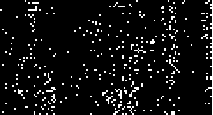
\includegraphics[width=120pt]{images/tm-sel-lc}}
  \hspace{6mm}
  \subfigure[colorized frame using Cheng's approach]{
\includegraphics[width=120pt]{images/tm-pred-lc}}\\
  \subfigure[grayscale
  image]{
\includegraphics[width=120pt]{images/tm-gray}} \hspace{6mm}
  \subfigure[selected pixels using
  our approach]{
\includegraphics[width=120pt]{images/tm-sel-lap}}
  \hspace{6mm} \subfigure[colorized image using
  our approach]{
\includegraphics[width=120pt]{images/tm-pred-lap}} \caption{\label{fig:tm-compare}
    Pixel selection and colorization on the first frame.}
\end{figure*}

